\documentclass{paper}
\usepackage{xeCJK}
\usepackage{listings}
\usepackage{hyperref}
\usepackage{amsmath,amssymb,amsthm}
\usepackage{xcolor}

%\lstset
%{
%    basicstyle=\ttfamily,
%    numbers=left,
%    % numberstyle=\tiny,
%    keywordstyle=\color[RGB]{0, 0, 255},
%    commentstyle=\color[RGB]{0, 128, 0},
%    frame=shadowbox,
%    rulesepcolor=\color{red!20!green!20!blue!20},
%    showspaces=false,
%    showstringspaces=false,
%    extendedchars=false,
%    showtabs=false,
%    tabsize=4, breaklines,
%    xleftmargin=2em,xrightmargin=2em, aboveskip=1em
%  }

\lstset{numbers=none,
  numberstyle=\scriptsize,
  flexiblecolumns=false,
  language=Haskell,
  frame=shadowbox,
  basicstyle=\ttfamily\small,
  breaklines=true,
  extendedchars=true,
  escapechar=\%,
  texcl=true,
  showstringspaces=false,
  keywordstyle=\bfseries,
  tabsize=4}

\setCJKmainfont{AR PL UKai CN}
\title{FOPL-Homework3}
\author{昂伟 PB11011058}


\begin{document}
%	\noindent {\bf Name : 昂伟 \quad Student Id : PB11011058 \quad FOPL-Homework3}
\maketitle

\section*{Problem 1}
\begin{itemize}
\item $	quicksort :: (Ord\ t)\Rightarrow [t] \rightarrow [t]$. 令$p::t$,由$(p:xs)$知,$quicksort$的参数类型为$[t]$;再由$(quicksort\ lesser) ++ [p]$知:$quicksort$的返回类型为$[t]$.由$<p, \geq p$知: $t$属于$Ord$类型类.

\item $	lesser :: (Ord\ t) \Rightarrow [t] $. 由$quicksort \ lesser$,且$quicksort :: (Ord\ t) \Rightarrow [t] \rightarrow [t]$知: $lesser :: (Ord\ t) \Rightarrow [t]$.

\item $	greater :: (Ord\ t) \Rightarrow [t]$. 推导过程类似于$lesser$.

\end{itemize}

\section*{Problem 2}
\subsection*{(a)}
	\begin{flushleft}
		$factRec :: (Int \rightarrow Int) \rightarrow Int \rightarrow Int$.\\
		由
		\begin{align*}
			case\ x\ &of\\
					 0 \ &\rightarrow \ 1\   \\
					\_\ &\rightarrow \ x\ *\ (g\ (x\ -\ 1))
		\end{align*}
		知: $$x::Int \eqno{(1)}$$
		由	
			$$ \ * \ :: Int \rightarrow Int \rightarrow Int$$\\
			$$ x\ *\ g (x\ -\ 1)$$
		知:$$g :: Int \rightarrow Int \eqno{(2)}$$
		由(1)(2)得:
			$$factRec :: (Int \rightarrow Int) \rightarrow Int \rightarrow Int$$		
		
	\end{flushleft}
\subsection*{(b)}
	\begin{flushleft}
 		$y :: (a \rightarrow a) \rightarrow a$.\\
 		令$$f :: a \rightarrow b,\ y :: (a \rightarrow b) \rightarrow b$$
 		由$$y\ f\ =\ f\ (y\ f)$$
 		且$$y\ f :: c, f(y\ f) :: b$$
 		知:$$b\ =\ c$$
 		又在$f(y\ f)$中$y\ f$作为$f$的参数且$y\ f :: c$\\
 		知:$$a\ =\ c$$
 		即得$$y :: (a \rightarrow a) \rightarrow a$$
 	\end{flushleft}

\subsection*{(c)}
	\begin{lstlisting}[language=Haskell]
	fibRec g = \n -> case n of 
						  0 -> 0 
						  1 -> 1 
						  n -> (g (n - 1)) + (g (n - 2)) 
	\end{lstlisting}

\subsection*{(d)}
	\subsubsection*{i}
			\begin{align*} 
				y\ (f) &= \lambda g.f(g\ g)(\lambda g.f(g\ g)) \\
					  &= f\ (\lambda g.f(g\ g)(\lambda g.f(g\ g)) \\
					  &= f\ (y\ f)
   			\end{align*}		
	\subsubsection*{ii} \emph{Haskell}是静态类型语言,不支持动态类型,所以y组合子定义无法通过{Haskell}静态类型推导系统,才会产生$T = T \rightarrow t_0$的类型错误.

\subsection*{(e)} 
	\begin{lstlisting}
	reduceRec g =  \f  \l -> case l of 
			[]  -> undefined 
			[x] -> x 
			(x:xs) -> f x (g f xs)
	\end{lstlisting}

\section*{Problem 3}
\subsection*{(a)} 
	\begin{lstlisting}
	myDecl = Fn "f" 
				(PatPair (PatVar "x") 
						 (PatVar "y"))
				(LetExp 
					(PatVar "z") 
					(App 
						(App 
							(IntExp 2) 
							(ExpVar "*")) 
						(ExpVar "x")) 
					(App 
						(App 
							(ExpVar "z") 
							(ExpVar "+")) 
						(ExpVar "y")))
	\end{lstlisting}
	
\subsection*{(b)} 见\href{./Inference.hs}{Inference.hs}
\subsection*{(c)}
	\begin{center}
	
		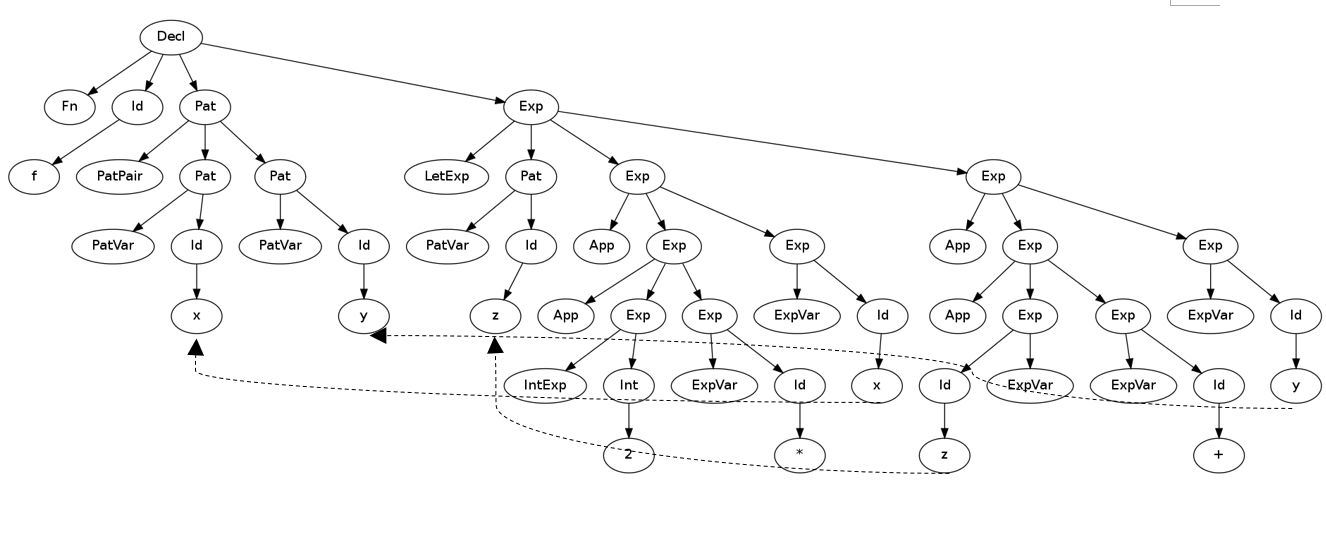
\includegraphics[width=1.3\textwidth]{./pro3_1.png}
		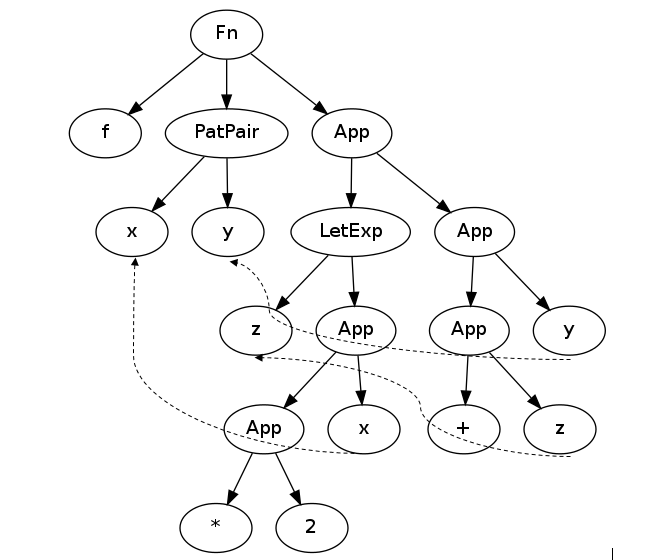
\includegraphics[width=0.8\textwidth]{./pro3_2.png}
	
	\end{center}
\subsection*{(d)}

	\subsubsection*{i}
		\begin{flushleft}	 
	 		由$Cond\ Exp\ Exp\ Exp$
			知:第一个Exp的类型必为$Bool$,第二个,第三个Exp的类型必须相同且为$Cond\ Exp\ Exp\ Exp$的类型.
	 	\end{flushleft}
	\subsubsection*{ii}
	\begin{center}
		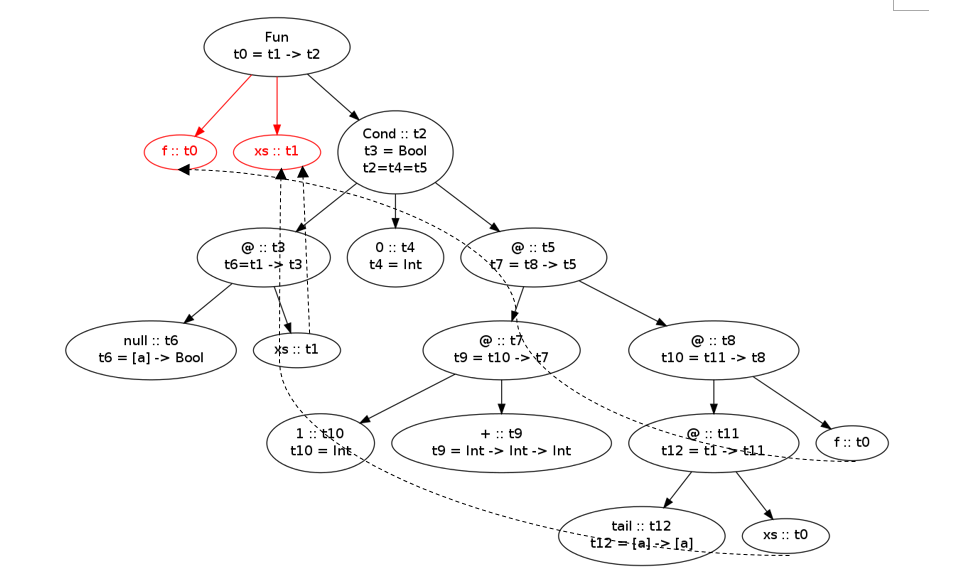
\includegraphics[width=0.8\textwidth]{./pro3_3.png}
	\end{center}
	\subsubsection*{iii} 
		\begin{align}
			t0 &= t1 \rightarrow t2  \\
			t2 &= t4 = t5  \\
			t3 &= Bool  \\
			t6 &= t1 \rightarrow t3  \\
			t6 &= [a] \rightarrow Bool \\
			t7 &= t8 \rightarrow t5  \\
			t10 &= t11 \rightarrow t8  \\
			t12 &= t1 \rightarrow t11  \\
			t12 &= [a] \rightarrow [a]  \\
			t9 &= t10 \rightarrow t7  \\
			t2 &= Int 
		\end{align}
		由(2)(11)知:
			$$ t2 = t4 = t5 = Int \eqno{(12)}$$
		由(4)(5)知:
			$$ t1 = [a]  \eqno{(13)} $$
		由(1)(12)(13)知:
			$$ t0 = [a] \rightarrow Int $$
	
\section*{Problem 4}
\subsection*{(a)} 
	\setcounter{equation}{0}
	\begin{align}
		t\_0 &= t\_3 \rightarrow t\_10 \\
		t\_3 &= (t\_1, t\_2)  \\
		t\_4 &= t\_9 \rightarrow t\_10  \\
		t\_9 &= (t\_7, t\_1)  \\
		t\_5 &= t\_2 \rightarrow t\_7  \\
		t\_5 &= Int \rightarrow String  \\
		t\_4 &= (String, String) \rightarrow String  
	\end{align}
	\begin{flushleft}
	由(5)(6)知:
			$$t\_2 = Int \eqno{(8)}$$ \\ 
			$$t\_7 = String \eqno{(9)} $$
	由(3)(7)知:$$t\_9 = (String, String) \eqno{(10)}$$
			$$ t\_10 = String \eqno{(11)}$$
	由(4)(10)知:$$t\_1 = String \eqno{(12)}$$
	由(12)(8)知:$$t\_3 = (String, Int) \eqno{(13)}$$
	由(11)(13)知:$$t\_0 = (String, Int) \rightarrow String \eqno{(14)}$$
	所以,$$g :: (String, Int) \rightarrow String$$
	\end{flushleft}
	
\subsection*{(b)}
	\begin{lstlisting}
	h :: (t_1, t_2) -> t_2
	y :: t_2
	xs :: [t_1]
	foldright h y xs :: t_2
	\end{lstlisting}
	
\subsection*{(c)}
	\begin{flushleft}
	我们想要$$f :: [Int] \rightarrow String$$
	但实际上由$$h = g :: (String, Int) \rightarrow String$$
	得,$$t_1 :: String,\ t_2 :: Int$$
	即$f :: [Int] \rightarrow [Int],\ y = "" :: String = t_2$矛盾.
	\end{flushleft}
\subsection*{(d)} 
	\begin{lstlisting}
	g(n, s) = Concats (show n, s)
	\end{lstlisting}

\section*{Problem 5}
\subsection*{(a)}
	\begin{lstlisting}[language=Haskell]
	-- Integer Comparison
	dCompInt :: CompD Int
	dCompInt = MakeCompD CompareInt
	
	-- List Comparison
	dCompList :: CompD a -> CompD [a]
	dcompList d = MakeCompD compList where
		compList [] [] = EQ
		compList (x:xs) [] = GT
		compList [] (y:ys) = LT
		compList (x:xs) (y:ys) = if (((?=) d x y) /= EQ)
								then ((?=) d x y)
								else (compList xs ys)
	\end{lstlisting}		
	
\subsection*{(b)}
	\begin{lstlisting}[language=Haskell]
	(?=) (dCompTuple (dCompInt, (dCompList dCompChar))) 
					 (length "Hello", "Hello") 
					 (length "World", "World"))
	(?=) dCompInt (length "Hello) (length "World")
	(?=) dCompList dCompChar "Hello" "World"
	(?=) dCompChar 'H' 'W'
	\end{lstlisting}

\subsection*{(c)} $f :: (Comp\ t) \Rightarrow [t] \rightarrow [t] \rightarrow Ordering$.由$length x$知: $x :: [t]$;又$xx\ ?=\ yy$知: $y :: [t]$;再由$f\ x\ y\ =\ xx\ ?=\ yy :: Ordering$,即得:$f :: (Comp\ t) \Rightarrow [t] \rightarrow [t] -> Ordering$.

\section*{Problem 6}
\subsection*{(a)} $MkEqD$是一个字典操作,用于重载时查询对应数据类型的相关函数调用操作;$===$从其第一个参数(即操作字典)中提取判别相等的函数.

\subsection*{(b)}
	\begin{lstlisting}[language=Haskell]
	instance MyEq a => MyEq (Tree a) where
		(===) (Leaf v1) (Leaf v2) = v1 === v2
		(===) (Node v1 tl1 tr1) 
			  (Node v2 tl2 tr2) = (v1 === v2) 
			  					& (tl1 === tl2) 
			  				    & (tr1 === tr2)
		(===) _ _ = False
	\end{lstlisting}

\subsection*{(c)}
	\begin{lstlisting}[language=Haskell]
	dMyEqTree :: MyEq a -> MyEq (Tree a)
	dMyEqTree d = MkMyEqD myEqTree where
		myEqTree (Leaf v1) (Leaf v2) = (===) d v1 v2
		myEqTree (Node v1 tl1 tr1) 
				 (Node v2 tl2 tr2) = 
								(===) d v1 v2 
								 & (myEqTree tl1 tl2) 
								 & (myEqTree tr1 tr2)
	\end{lstlisting}
	
\subsection*{(d)} 因为函数$cmp$声明使用了qualified type \textit{MyEq a}.为了能正确的调用类型$a$所对应的$(===)$函数,编译器必须对$cmp$进行改写,即加入$a$类型数据所对应的操作字典.

\subsection*{(e)} 
	\begin{lstlisting}[language=Haskell]
	cmp' :: MyEq a -> a -> a -> String
	cmp' d t1 t2 = if (===) d t1 t2 
				   then "Equal"
				   else "Not Equal"
	result' = cmp' (dMyEqTree dMyEqInt) test1 test2				
	\end{lstlisting}
	
\end{document}
